\section{The Numerical Method}
\label{sec:related}

Since local optimality does not guarantee global optimality, a fundamental concern in global optimization is getting stuck at a local optimum point \cite{dekkers}. In order to avoid and overcome this, a specific class of stochastic optimization is used, which is simulated annealing. Simulated annealing originates from the physical annealing process that is well known in condensed matter physics \cite{dekkers}. Physical annealing is a thermal process where the heating and slow cooling of a metal in a heat bath brings it into a more uniformly crystalline state where the free energy takes its global minimum. The role of temperature in physical annealing is to allow the particles to reach higher energy states in order to overcome energy barriers that would force them into local minima \cite{neumaier}. \\
\hspace*{3mm}In greater detail, a state with energy level $E_1$ is compared to a state with energy level $E_2$, which is obtained by moving one of the particles into another location by a small displacement. $E_2$ is only accepted if the movement of the particle brings the system in a state of lower energy (i.e. $E_2-E_1\leq0$). If this is not the case, a movement to a state of higher energy $E_2$ (also called a deterioration) is only accepted with probability 
$e^-{\frac{(E_2-E_1)}{kT}}$, where $k$ is the Boltzmann constant and $T$ is the temperature \cite{dekkers}. However, the probability of accepting these deteriorations descends slowly towards zero as this process continues. Thus, the repetition of this process for a large enough number of particle movements using this stochastic acceptance criterion for deteriorations make it possible to overcome becoming stuck at local minima and leads to a (near) global minima \cite{dekkers}.\\
\hspace*{3mm}In 1983, Kirkpatrick, Gellatt and Vecchi applied the physical annealing of metal with combinatorial minimization by replacing energy with a cost function and the movement of the particles in the physical system became analogous to a trial in the combinatorial minimization problem \cite{dekkers}. This algorithm proves to have many benefits when applied to combinatorial minimization problems including guarantee of convergence to global minimum, generally applicable to the cost function and easy to implement with good performance \cite{dekkers}. \\
\hspace*{3mm}The approach of the simulated annealing algorithm is to generate homogeneous Markov chains of finite length at a finite sequence of descending values of the control parameter \cite{dekkers}. The cooling schedule consists of a set of parameters that controls the convergence of the algorithm, as listed below: \\
\begin{itemize}
\item initial value of the control parameter $c$ 
\item a decrement function for decreasing the value of the control parameter $c$
\item a stop criterion
\item a finite length, $L$, of each Markov chain\\ \cite{dekkers}   
\end{itemize}

The parameters of the cooling schedule are described below in more detail.

\subsection{Initial value of the control parameter ($c_0$)}

The basic assumption regarding the initial value of the control parameter is that $c_0$ should be sufficiently large such that approximately all transitions are accepted at this value. If we let $\chi(c)$ denote the ratio between the number of accepted transitions and number of accepted transitions along the Markov chain at $c$. The problem of determining $c_0$ can be posed in terms of requiring
the initial acceptance ratio $\chi_0=\chi(c_0)$ to be close to 1.

The authors of \cite{dekkers} propose that $c_0$ be determined by the following scheme: The objective function $f(\vect{x})$ is sampled
$m$ times with $\vect{x} \sim \mathrm{Uniform}\left( \mathcal{S}\right)$. Let $\Delta f = f(\vect{y}) - f(\vect{x})$, and
$\Delta f^+ = \left\lbrace \Delta f : \Delta f > 0 \right\rbrace$. Let $m_1$ denote the number of accepted transitions, with
$m=m_1+m_2$, and let $\overline{\Delta f^+}$ be the average values of $\Delta f_{xy}$ for which $\Delta f_{xy}>0$

\begin{equation}
\label{eq:3-2}
    c_0 = \overline{\Delta {f}^+} \, \Bigg(\ln \dfrac{m_2}{m_2 \chi_0+(1-\chi_0)m_1} \Bigg)^{-1} 
\end{equation}

In practice, \cref{eq:3-2} was found to be problematic. The logarithm can result in a negative $c_0$ which does not make sense.
Furthermore, if $m$ is not sufficiently large, $c_0$ exhibits very high variance. This occurs because the mean in 
$\overline{\Delta f^+}$ is very sensitive to extreme values. Quick examination of the histograms of $\Delta f^+$ of the Rosenbrock
test function suggested that $\Delta f^+$ is heavy-tailed.

Instead let's suppose we want the $\chi_0$-th quantile transition to have a high ($p=0.9)$ probability of being accepted. 
\Cref{fig:acceptance} shows that $\exp -\Delta f / c$ maps $\Delta f$ onto a probability. If we let $k=\chi$-th quantile of the
$\Delta f^+$ values, we can determine $c_0$ with


\begin{equation}
    \label{eq:schedule_init}
    \exp - \frac{k}{c_0} \geq p \implies c_0 = -\frac{k}{\log p}
\end{equation}

\begin{figure}
    \centering
    \textbf{Affect of $c$ on acceptance probability}
    %\caption{}
    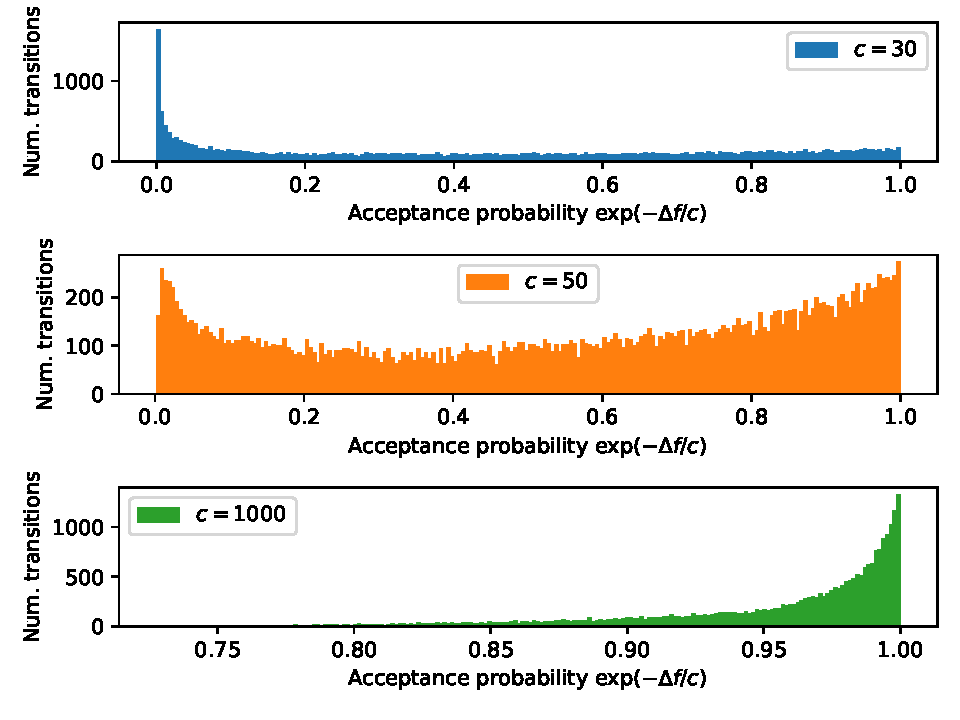
\includegraphics[scale=0.5]{figures/fig33.pdf}
    \label{fig:acceptance}
    
  \caption{Using the Rosenbrock function, 50,000 transitions were computed. Among those, the positive transitions were selected and the exponential function $exp(-\Delta f/c)$  was applied and used as the acceptance criterion. Using three different $c$ values of 30, 50 and 1000, it is shown that a greater value of $c$ leads to more transitions given a higher probability of being accepted.}
\end{figure}

\subsection{Decrement of the control parameter}
The decrement function is used to decrease the value of $c$\\
The new value of $c$, $c'$ is calculated by:
\begin{equation}\label{eq:c_dec}
    c'=c \, \Bigg(1+\dfrac{c\ln(1+\delta)}{3\sigma (c)}\Bigg)^{-1} 
\end{equation} 
where $\sigma(c)$ is the standard deviation of the values of the cost function of the points of the Markov chain at $c$ and the constant $\delta$ is the distance parameter that determines the speed of the decrement of the control parameter $c$ \cite{dekkers}.

Particular care must be given towards the $\sigma(c)$ term in the denominator of \cref{eq:c_dec}. Especially when $c$ is small, towards
the later stages of the annealing schedule, a Markov chain at the current $c$ can fail to make any transitions. In such situations,
$\sigma(c) = 0$, and we have both a divide-by-zero exception, and $c$ can be set to 0 prematurely, which has the result of triggering
the stop condition, before a good solution is reached.

One way to address this issue is to repeatedly sample a Markov chain until some minimum number of transitions are performed. Due to
descent direction component of point generation alternative B, the Markov chain will usually make at least one transition, even
if it is very small, thus avoiding the divide-by-zero problem.

\begin{figure}[h]
    \centering
    \caption{Cooling schedule for Branin}
    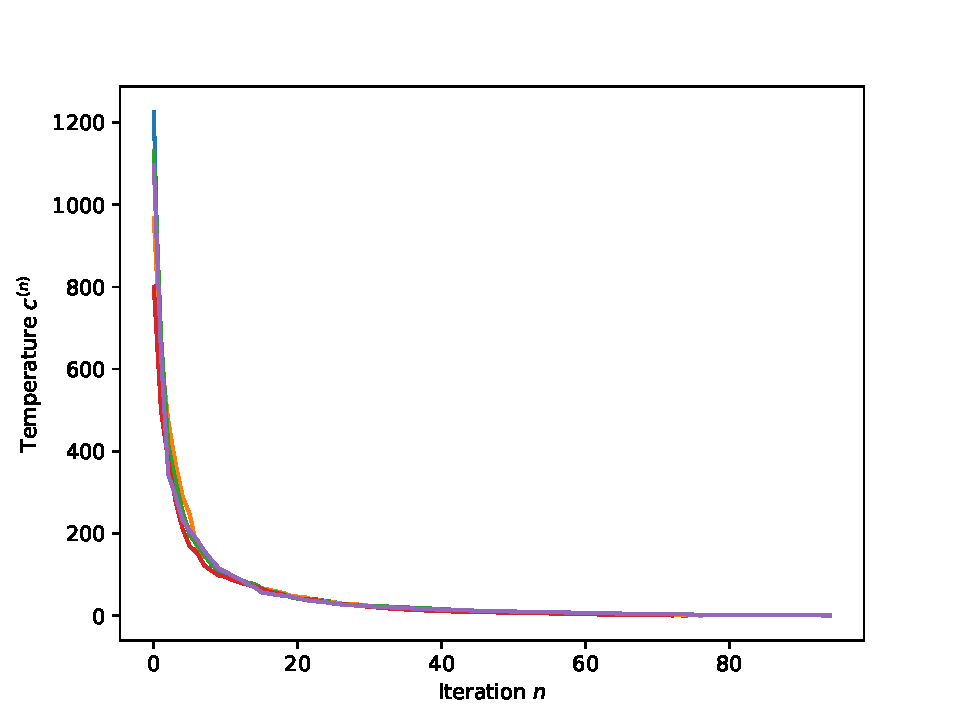
\includegraphics[scale=0.42]{figures/fig31-branin.pdf}
    \label{fig:512}
\end{figure}

\begin{figure}[h]
    \centering
    \caption{Cooling schedule for Goldstein-Price}
    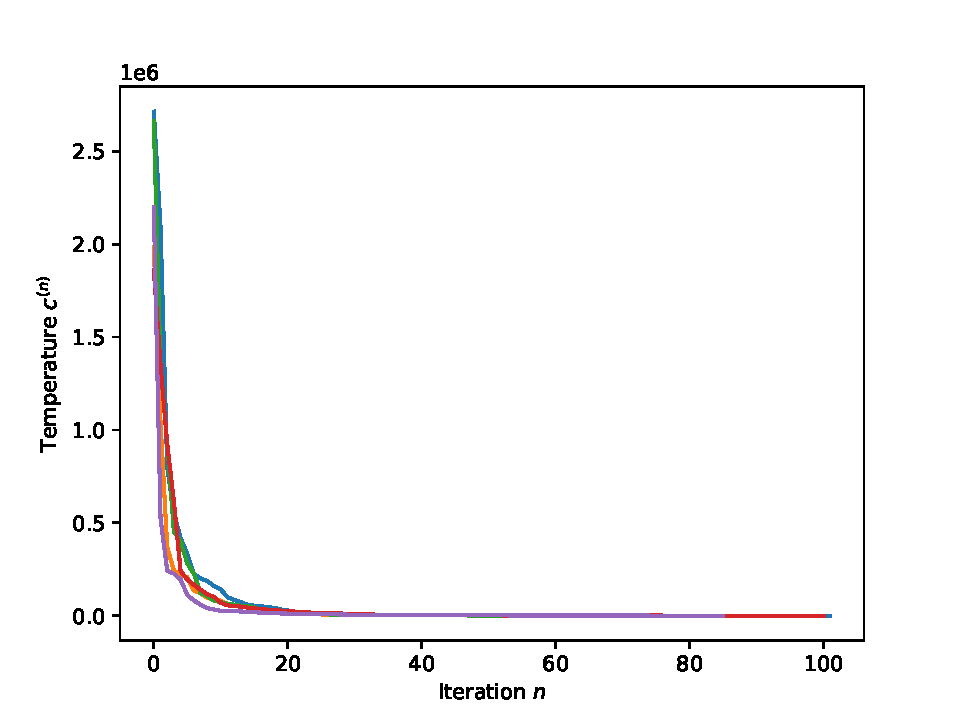
\includegraphics[scale=0.42]{figures/fig31-goldstein_price.pdf}
    \label{fig:512}
    \caption*{Figure 2 and Figure 3 represent an example Cooling Schedule for Branin and Golden-Price respectively, where each colour on the curve represents a different run, for 4 total runs.}
\end{figure}

\subsection{Stop condition}

Particular care needs to be given to devising an appropriate stopping condition.
First, let $\overline{f}(c_0)$ denote the mean value of the points in the initial Markov chain, and $\overline{f}(c)$ denote
the average values of the points in the chain at $c$. Then $\overline{f_s}(c)$ is the smoothed value of $\overline{f}$
over a number of chains in order to reduce fluctuations of $\overline{f}(c)$. In practice the smoothing is applied
using a small smoothing parameter $0 < \gamma < 1$ and

\begin{equation}
    \label{smoothing}
    \begin{array}{c}
    \overline{f_s}^{(n+1)} = \gamma \overline{f}^{(n+1)} + (1-\gamma) \overline{f_s}^{(n)} \\
    \\
    \overline{f_s}^{(0)} = \overline{f}^{(0)} \\
    \end{array}
\end{equation}

The algorithm is terminated if:
\begin{equation}
\label{eq:stop_cond}
    \Bigg|\frac{d \overline{f_s}(c)}{dc} \frac{c}{\overline{f}(c_0)} \Bigg| < \epsilon_s 
\end{equation}

where $\epsilon_s$ is the stop parameter, a small positive real number. The derivative in \cref{eq:stop_cond}
is simply calculated using a finite difference method \cite{dekkers}.
 
%\begin{itemize}
%\item$\overline{f}(c_0)$ is the mean value of the points found in the initial Markov chain
%\item $\overline{f_s}(c)$ is the smoothed value of $\overline{f}$ over a number of chains in order to reduce %fluctuations of $\overline{f}(c)$ and
%\item $\epsilon_s$ is the stop parameter, a small positive real number.
%\end{itemize}

\subsection{Length of the Markov chains}
Let $n$ be the dimension of $S$ and let $L_0$ be a constant called the standard length. Then 
\begin{equation}
    L=L_0 \cdot n     
\end{equation}
is the length of the Markov chain, which must be sufficiently large in order to enable the algorithm to explore the neighbourhood of a given point in all directions \cite{dekkers}. \vspace{5pt}

A pseudo-code for the algorithm can be found in \textbf{Algorithm \ref{algo:sa}}.


\begin{algorithm}
\setstretch{1.4}
\caption{Simulated Annealing}\label{algo:sa}
\vspace{8pt}
\nosemic
\SetAlgoLined
\KwIn{$f:\mathcal{S} \longrightarrow \Real, \nabla f, \mathcal{S}, N, \epsilon_s, \tau, \gamma$}

\end{algorithm}

%$f^\star \longleftarrow \infty$\;

%\;

%\For{$n\in \left\lbrace 1,\ldots, N\right\rbrace$}{
%$\vect{x}_0 \longleftarrow \mathrm{Uniform}\left(\mathcal{S}\right)$ \Comment*{random sample init. point}

%$x_l = \texttt{steepest\_descent}(f, \nabla f, \vect{x}_0, \tau)$ \;

%\If{$f(\vect{x}_l) \leq f^\star$}{
%    $f^\star \longleftarrow f(\vect{x}_l)$ \;
%    
%    $\vect{x}^\star \longleftarrow \vect{x}_l$ \;
%}

%\uIf{$n=0$}{
%    $f^\star_s \longleftarrow C$ \Comment*{$0< C \in\Real$ to prevent 0}
%    $f^\star_s^{(0)} \longleftarrow f_s^\star$ \;
%} \uElse{
%    $f^\star_s^{(0)} \longleftarrow f^\star_s$ \;
%    $f^\star_s = \gamma f^\star + (1-\gamma)f^\star_s^{(0)}$
%    \;
%    \Comment{Stop when smoothed improvement reaches 0}
%    $\Delta_s = f^\star_s^{(0)} - f^\star_s$ \;
%    
%    \Comment{Check stop condition}
%    \If{ $\Delta_s \leq \epsilon_s$}{
%        \KwOut{Solution found $\vect{x}^\star$}
%    }
%}

%\;
%\KwOut{Failed to find solution in $N$ iterations, $\vect{x}^\star$}\;
%}
%\end{algorithm}

%\begin{algorithm}[t]
%\caption{\textsc{Simulated Annealing}}
%\begin{algorithmic}
%\STATE begin
%\STATE "initialize $(c,x)$;"
%\STATE stopcriterion := false;
%\WHILE{stopcriterion = false} 
%\STATE begin
%\FOR{$i$:=1 \TO $L$}
%\STATE begin
%\STATE "generate $y$ from $x$";
%\IF{$f(y)-f(x) \leq 0$}
%\STATE accept
%\ELSIF{$\exp{(-(f(y)-f(x))/c)} > \textsc{random}[0,1)$}
%\STATE accept;
%\IF{accept}
%\STATE $x:=y$
%\ENDIF
%\ENDIF
%\STATE "lower c"
%\ENDFOR
%\ENDWHILE
%\end{algorithmic}
%\label{algo:sa}
%\end{algorithm}

\subsection{Generation of Points} 
\label{sec:gen-points}
There are several ways to generate new points from a given point and two alternatives are used for the purposes of this project, Alternative A and Alternative B:
\begin{enumerate}[label=\textbf{(\Alph*)}]
    \item A uniform distributions on $S$:
    \begin{equation}
        g_{xy}=\frac{1}{m(S)} 
    \end{equation}
A disadvantage about Alternative A is that no structural information about function values is used \cite{dekkers}.
    \item Either a point is drawn from a uniform distribution over $S$ or a step is made into a descent direction from the current point:
    \begin{equation}
    g_{xy}=\begin{cases}
          LS(x) \quad &\text{if} \, w>t \\
          \dfrac{1}{m(S)} \quad &\text{if} \, w \leq t \\
     \end{cases} 
    \end{equation}
    where $t$ is a fixed number in the interval [0,1) and $w$ is a random number from $U$[0,1). LS(x) is a Local Search procedure (i.e Steepest Descent Method) that generates a point $y$ in a descent direction of $x$. \cite{dekkers}

\end{enumerate}




 
